%%%%%%%%%%%%%%%%%%%%%%%%%%%%%%%%%%%%%%%%%
% Template formal para se utilizar na equipe de propulsão e tecnologia aeroespacial (EPTA)
% LaTeX Template
% Version 1.0 (16/07/2019)
%
% This template was downloaded from:
%
% Original author:
% Peter Wilson (herries.press@earthlink.net) with modifications by:
% Vel (vel@latextemplates.com)
% Vel (feliperibeiro.ufu@gmail.com)
% Vel (mairaf_miranda@hotmail.com)
%
% License:
% CC BY-NC-SA 3.0 (http://creativecommons.org/licenses/by-nc-sa/3.0/)
%
% Conselhos para se lidar com este template:
% - Evitar alterar códigos referentes à formatação, com exceção de se copiar e colar
%          o código para exibição de imagens, tabelas e equações.
% - Procurar sempre manter as imagens utilizadas no documento em uma pasta dedicada,
%          de forma que, ao se referenciar a imagem, se referencie o caminho para 
%          ela, como feito com a "imagem_de_missao".
%
%
%%%%%%%%%%%%%%%%%%%%%%%%%%%%%%%%%%%%%%%%%

%----------------------------------------------------------------------------------------
%	Pacotes utilizados.(evitar mudar, se for necessária alguma mudança, comunicar gerencia)
%----------------------------------------------------------------------------------------

\documentclass[a4paper, 12pt,  oneside,a4paper,english,french,spanish,brazil]{book}     % Para folha A4, default 11pt tamanho
\usepackage[utf8]{inputenc}                                               % Acentos
\usepackage[brazil]{babel}                                                % Biblioteca para português
\usepackage{amssymb}                                                      % Biblioteca para símbolos
\usepackage{graphicx}                                                     % Biblioteca para figuras
\usepackage{tikz}                                                         % Pacote gráfico
\usepackage{amsmath}                                                      % Biblioteca para símbolos
\usepackage[T1]{fontenc}                                                  % encode para acentos 
\usepackage{fouriernc}                                                    % New Century Schoolbook font
\usepackage{xcolor}                                                       % Controle de cores
\usepackage[many]{tcolorbox}                                              % Controle de cores
\usepackage{amsthm}                                                       % Suporte matemático ams
\usepackage{physics}                                                      % Suporte em notações
\usepackage{gensymb}                                                      % Suporte em notação
\usepackage{amsfonts}                                                     % Suporte em fontes ams
\usepackage[left=1.00cm, right=1.00cm, top=3cm, bottom=2.50cm]{geometry}  % Parâmetros geométricos
\usepackage{caption}                                                      % Legenda para imagens
\usepackage{subcaption}                                                   % Legenda para figuras múltiplas
\usepackage{capt-of}                                                      % Suporte com legendas
\usepackage{float}                                                        % Suporte para maiores floats  
\usepackage[figurename=Fig.]{caption}                                     % Suporte 2 títulos legendas
\usepackage{tabularx}                                                     % suporte com tabelas
\usepackage{ragged2e}                                                     % suporte localização texto
\usepackage{mathrsfs}                                                     % Fontes para equações
\usepackage{makecell}                                                     % Formatação de tabelas
\usepackage{textpos}                                                      % Facilita posicionamento de forma absoluta
\usepackage[hyphens]{url}                                                 % Possibilita uso de hífen em links
\usepackage[makeroom]{cancel}                                             % Desconsidera limites para retas
\usepackage{empheq}                                                       % Possibilita emoldurar fórmulas
\usepackage[colorlinks=true,linkcolor=blue,urlcolor=blue,bookmarksopen=true, bookmarksnumbered, pdfencoding=auto]{hyperref}                                               % links clicáveis em PDF
\usepackage{fancyhdr}                                                     % Ajuda na criação de footers e headers
\usepackage{siunitx}                                                      % General suporte
\usepackage{enumitem}                                                     % Controle sobre layout
\usepackage{cancel}                                                       % Riscar coisas
\usepackage{bookmark}                                                     % Hiperlink em PDF
\usepackage{versions}                                                     % Devido às versões
\usepackage[pages=some,scale=1,angle=0,opacity=1]{background}             % Imagem de Background
\usetikzlibrary{decorations.pathmorphing}                                 % Permite utilização direta fonte abaixo
\usetikzlibrary{shapes.callouts,positioning}                              % Balões   
\usetikzlibrary{shapes.geometric,arrows,shadows}                          % flechas
\usepackage{frcursive}                                                    % Fonte cursiva
\usepackage{multirow}                                                     % Suporte tabelas

\setlength\parindent{3ex}                                                 % Parâmetro geométrico
\setlength{\parskip}{0.25em}                                              % Parâmetro geométrico
\setlength{\fboxsep}{10pt}                                                % Espaço ao redor dos quadros
\definecolor{zelena}{RGB}{0,100,0}                                        % Define cores em estruturas
\tcbuselibrary{theorems}                                                  % Cor nas caixas                           
\tcbuselibrary{breakable}                                                 % Particiona coisas
\pagestyle{fancy}  
\fancyhead[RO , RE]{\footnotesize 
	\begin{minipage}[b]{0.435\linewidth}\flushright\leftmark\end{minipage}}  % cabeçalho direito ímpar=título do capítulo
\fancyhead[LO , LE]{\footnotesize 	
	\begin{minipage}[b]{0.435\linewidth}\flushleft\rightmark\end{minipage}} % cabeçalho esquerdo = nome da seção
\fancyfoot[CE,CO]{\thepage}                                               % Nota de pé
\allowdisplaybreaks                                                       % Possibilita alguns comandos de controle
\setcellgapes{5pt}                                                        % Formatação de tabelas
\definecolor{eggshell}{rgb}{0.94, 0.92, 0.84}                             % Definição de cor 



\setlength\headheight{27.05003pt}
\renewcommand\headrule{\hrulefill
	\raisebox{10.1pt}[-10pt][-10pt]{\plogo}\hrulefill}                      % Headers
\newcommand{\plogo}{\fbox{  $EPTA$   }}                                   % sigla equipe 
\newcommand\BackImage[2][scale=1]{\BgThispage\backgroundsetup{
		contents={\includegraphics[#1]{#2}}}}                             % cria a função background
\newtcbox{\caixaeq}[1][]{nobeforeafter,math upper,tcbox raise base,enhanced,
	colframe=black!50!black,colback=eggshell!40!white,arc=4pt,	
	boxrule=1pt,drop fuzzy shadow,#1}                                     % Moldura para fórmulas

\DeclareMathOperator{\tg}{tg}                                             % Declara construção mat. 
\DeclareMathOperator{\cotg}{cotg}                                         % Declara construção mat.
\usepackage{csquotes}
\usepackage{adjustbox}
\usepackage{plantuml}
\usepackage{epstopdf}
\epstopdfDeclareGraphicsRule{.svg}{pdf}{.pdf}{
    inkscape -z --file=#1 ==export-pdf=\OutputFile
}

%%%%%%%%%%%%%%%%%%%%%%%%%%%%%%%%%%%%%%%%%
\frontmatter
\date{}
% \thispagestyle{empty}
\date{\today}
\sloppy
\usepackage{eso-pic}
\newcommand\BackgroundPic{%
\put(0,0){%
\parbox[b][\paperheight]{\paperwidth}{%
\vfill
\centering

\includegraphics[width=\paperwidth,height=\paperheight,%
keepaspectratio]{midia/epta_projeto_template}%
\vfill
}}}
\lstdefinestyle{sharpc}{language=[Sharp]C, frame=lr, rulecolor=\color{blue!80!black}} % Style of code
\lstset{
extendedchars=true,
literate={á}{{\'a}}1 {ã}{{\~a}}1 {é}{{\'e}}1 {ç}{{\c{c}}}1 {ú}{{\'u}}1 {ó}{{\'o}}1 {à}{{\`a}}1,
language=csh,
basicstyle=\footnotesize\ttfamily,
numbers=left,
numberstyle=\tiny,
numbersep=5pt,
tabsize=2,
extendedchars=true,
breaklines=true,
frame=b,
stringstyle=\color{blue}\ttfamily,
showspaces=false,
showtabs=false,
xleftmargin=17pt,
framexleftmargin=17pt,
framexrightmargin=5pt,
framexbottommargin=4pt,
commentstyle=\color{black},
morecomment=[l]{//}, %use comment-line-style!
morecomment=[s]{/*}{*/}, %for multiline comments
showstringspaces=false,
morekeywords={ abstract, event, new, struct,
as, explicit, null, switch,
base, extern, object, this,
bool, false, operator, throw,
break, finally, out, true,
byte, fixed, override, try,
case, float, params, typeof,
catch, for, private, uint,
char, foreach, protected, ulong,
checked, goto, public, unchecked,
class, if, readonly, unsafe,
const, implicit, ref, ushort,
continue, in, return, using,
decimal, int, sbyte, virtual,
default, interface, sealed, volatile,
delegate, internal, short, void,
do, is, sizeof, while,
double, lock, stackalloc,
else, long, static,
enum, namespace, string},
keywordstyle=\color{blue},
identifierstyle=\color{red},
backgroundcolor=\color{white},
}

%----------------------------------------------------------------------------------------
%    INÍCIO DO DOCUMENTO    (a partir daqui pode editar sem grandes complicações)
%----------------------------------------------------------------------------------------
\begin{document} 

%----------------------------------------------------------------------------------------
%	PÁGINA DE TÍTULO
%----------------------------------------------------------------------------------------

\begin{titlepage} % Suprime cabeçalhos e notas na base da folha.

	\AddToShipoutPicture*{\BackgroundPic}
	\begin{minipage}[h!]{0.36\textwidth}
        \phantom{..}
    \end{minipage} 
    \begin{minipage}[h!]{0.6\textwidth}
	
		\centering % centraliza os textos na página
	
		\scshape % Usa formatação pequena 
	
		%------------------------------------------------
		%	Título
		%------------------------------------------------
	
		\rule{\textwidth}{1.6pt}\vspace*{-\baselineskip}\vspace*{2pt} % Linha horizontal grossa
		\rule{\textwidth}{0.4pt} % Linha horizontal fina
	
		\vspace{0.75\baselineskip} % espaço sobre o título
	
		{\LARGE EPTA Entertainment\\} % Título
	
		\vspace{0.75\baselineskip} % espaço abaixo do título
	
		\rule{\textwidth}{0.4pt}\vspace*{-\baselineskip}\vspace{3.2pt} % Linha horizontal fina
		\rule{\textwidth}{1.6pt} % Linha horizontal grossa
	
		\vspace{2\baselineskip} %espaço em branco abaixo do título
	
		%------------------------------------------------
		%	Subtítulo
		%------------------------------------------------
	
		Neste documento encontra-se o plano de desenvolvimento que se refere à criação da versão $1.0$ do aplicativo EPTA Space Program, desenvolvido pela EPTA Entertainment.% descrição adicional (sub-título)
	
		\vspace*{3\baselineskip} % espaço abaixo do subtítulo
	
		%------------------------------------------------
		%	Autores(s)
		%------------------------------------------------
	
		Desenvolvido por
	
		\vspace{0.8\baselineskip} % Espaço antes de autores
		
        {
        Felipe J. O. Ribeiro \\ 
        Mateus da Silva Fernandes \\ 
        Olavo Caetano Inácio \\
        Pedro Guilherme R. V. de Melo
        } % Lista de autores (ordem alfabética)
        
		
        \vspace{0.8\baselineskip} % Espaço após os autores
	
		\textit{Universidade Federal de \\ Uberlândia} % Entidades envolvidas
	
		\vspace{12.8\baselineskip} % Espaço (diminuir se houver mais autores)
	
		{\large Equipe de Propulsão e Tecnologia Aeroespacial} % equipe
		
		\vspace{0.3\baselineskip} % Espaço embaixo da logo
		
		EPTA Space Program - Versão 1.0 % Núcleo análogo
		
		\vspace{0.3\baselineskip} % Espaço embaixo da logo
		
		\today % Data de compilação
		
	\end{minipage}



\end{titlepage}

%----------------------------------------------------------------------------------------
%   Abstract...     (Um resumo do que será tratado em todo o texto)
%----------------------------------------------------------------------------------------
{
	\thispagestyle{empty}     % Sem numeração no abstract
	
	{\LARGE Resumo} % Abstract (grande)
    \vspace{1cm}
	
    Neste documento encontram-se as práticas adotadas no desenvolvimento da versão $1.0$ do aplicativo Epta Space Program. O programa já havia sido lançado na google play em meados de 2017, mas ele foi retirado do ar devido a questões burocráticas (ausência de uma política de privacidade). 

    Nesta etapa de desenvolvimento a equipe atualizará o jogo para a versão mais recente do unity.
    Também revisará o work flow uma vez que na versão de 2017 estava impossível de escalar e inviável de manter devido a más práticas de programação.
    Como resposta a isso, a sub área se propôs a revisar todos os padrões de desenvolvimento de forma a estar conforme com as mais altas recomendações desta indústria.


    As funções base do aplicativo são:

    \begin{description}[font=$\bullet$~\normalfont\scshape]
        \item [Tela inicial] Desenvolvimento da tela inicial com animações. Que não precise iniciar o jogo pausado.
        \item [3 fases] Três etapas distintas de jogo. (céu azul, extratosfera, espaço)
        \item [Fase final] A certa altura (a determinar), o player tem a opção de de ir para a lua. (o conteúdo será adicionado posteriormente. Mas por hora o player recebe uma mensagem de congratulações)
        \item [Morte] Som e efeito visual de explosão no momento de morte.
        \item [Arcade] Mecânica base do jogo mantém-se arcade, com rolagem para cima com obstáculos e replay ágil.
    \end{description}

    As features que espera-se que estejam presentes no jogo na data de estreia são:

    \begin{description}[font=$\bullet$~\normalfont\scshape]
        \item [Propaganda] As propagandas tipo banner e tipo Intersticial devem ser implementadas novamente.
        \item [Versão paga] Deve haver uma versão sem propagandas e que é paga. (preço a determinar)
        \item [Tabela Info] Tabela de informações sobre a equipe no menu opções.
        \item [Volume] Deve ser possível ajustar o volume.
        \item [Salvar] A melhor pontuação do jogador deve ser salva localmente, assim como o volume.
        \item [Assests reutilizados] Serão utilizados os assets do antigo lançamento. Novos devem ser feitos conforme necessidade.
        \item [Alturas reais] As alturas de mudança de fase devem ser consistentes com o mundo real.
        \item [Dificuldade crescente] O sistema de dificuldade deve ser implementado de forma a permitir razoável controle em função de fase e tempo.
    \end{description}

    A metodologia adotada para a criação do APP tem duas etapas importantes: Até o término da versão $1.0$ será adotada uma metodologia em cascata, nesta que é a etapa de pré lançamento, onde se dividirão as features a implementar em uma ordem lógica de execução. 
    Datas para pontos chave no desenvolvimento serão determinadas seguindo o padrão industrial (pre-alpha : $0.5.0$, alpha : $0.6.0$, beta-1 : $0.7.0$, beta-2 : $0.8.0$, ..., release : $1.0.0$), onde cada uma terá um objetivo e uma lista de requerimentos a serem atendidos.
    Em seguida, após lançado, será adotada a metodologia ágil para desenvolvimento contínuo de atualizações e melhoramentos conforme necessário. Esse será chamada de etapa contínua de pós lançamento.

    Será implementado um ciclo de desenvolvimento completamente integrado à ferramente Git de controle de versão e à página GitHub (\url{https://github.com/Epta-space/EPTA_SPACE_PROGRAM}), onde o jogo será salvo em cloud em um repositório privado.
    Assim, essas ferramentas servirão para possibilitar o desenvolvimento em grupo do código fonte, além de também ser uma forma de quantificação da produtividade, uma vez que o controle do número de commits é uma métrica importante no acompanhamento das atividades.
    Mais detalhes podem ser encontrados na descrição das etapas de desenvolvimento do pré lançamento.

    A criação do produto mínimo viável já foi feita na primeira versão do jogo, motivo pelo qual não temos a etapa MVP neste texto. 
    Apesar disso será inserida aqui alguma documentação sobre esse processo nos capítulos iniciais.
    O desenvolvimentos que ocorreram anteriores a esse relatório são o motivo, também, da enumeração das etapas começarem em $0.5$.
    Nos capítulos iniciais também será dada uma detalhada noção do estado atual do aplicativo assim como algumas informações sobre como foi o desenvolvimento até então.
    Tudo que foi feito até o momento foi desenvolvido durante o ano corrido de 2020, com exceção dos assets que vem da versão anterior.

    Dentre as informações do estado atual do aplicativo serão listados os scripts que existem atualmente em formato UML e por escrito, a estrutura de arquivos no projeto unity e a estrutura de Prefabs.
    Estas estruturas também já atendem a padrões de projeto sugeridos online e facilitam o desenvolvimento do controle de versão via Git, além de organizar as informações para facilitar o acesso e aumentar a escalabilidade.

    Próximo ao fim do documento também serão apresentadas algumas propostas de melhoramento na etapa ágil de lançamento, isso é, após a primeira versão do programa ser lançada na Google Play. Isso mostra as possíveis rotas que a subárea tomará no futuro, após o começo da etapa de desenvolvimento contínuo.

	\vspace{1cm}
	{\large Palavras chave:} {\small Desenvolvimento de Software, aplicativo, android, jogo, google play.}

}
%----------------------------------------------------------------------------------------
%	Desenvolvimento...
%----------------------------------------------------------------------------------------

\tableofcontents          % Índice
\thispagestyle{empty}     % Sem numeração na página do índice
\listoffigures            % Lista de figuras 
\thispagestyle{empty}     % Sem numeração na página da lista de imagens
\mainmatter

\chapter{O desenvolvimento até aqui}

    O início deste projeto ocorreu no começo do primeiro semestre de 2018. Um grupo de membros se juntou no desenvolvimento do aplicativo como uma nova proposta de angariação de fundos para a equipe. 
    Observou-se o potencial do mercado de aplicativos global, que cresce consistentemente ao longo dos anos.
    Além disso pensou-se na oportunidade de se aprofundar no desenvolvimento de software e o aprendizado que isso traria.

    Ao longo do ano o aplicativo foi desenvolvido e finalmente lançado em dezembro de 2018. Ele foi baixado em mais de 40 países e mais de 800 vezes, com uma avaliação média de $4.88$ estrelas de $5$ (Fig.\ref{grafico_inicial}): 

    \begin{figure}[h!]
        \centering
        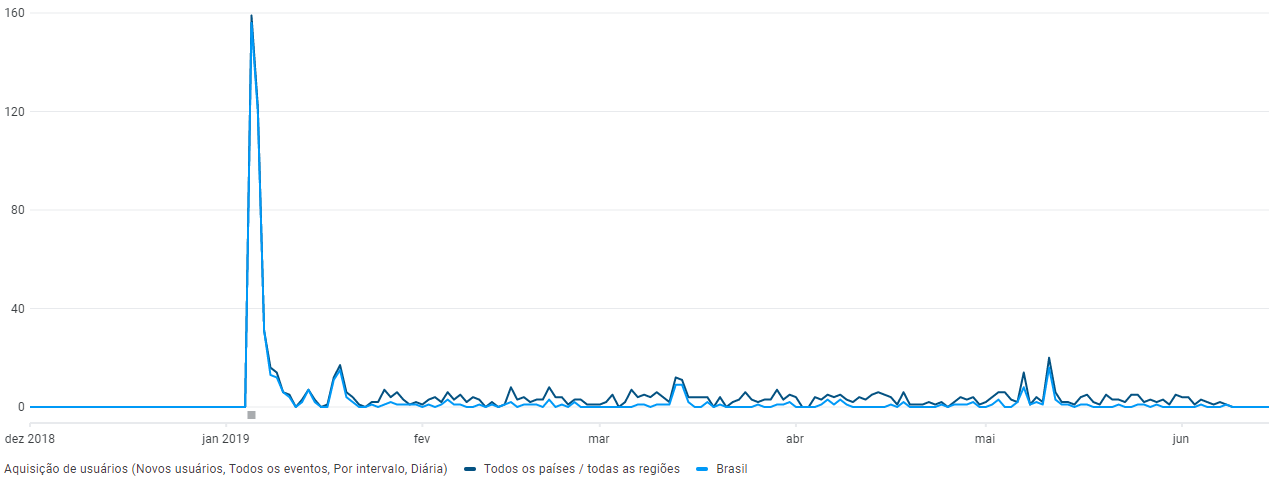
\includegraphics[trim = {0cm 0cm 0cm 0cm}, clip , angle=0, scale=0.55]{midia/users_global.png}
        \caption{Downloads do aplicativo distribuídos no tempo.}
        \label{grafico_inicial}
    \end{figure}

    Em julho de 2019 o aplicativo foi retirado da Play Store devido à ausência de uma politica de privacidade. Isso deu início a um longo hiato no desenvolvimento que só foi retomado no início de 2020. 
    
    A estratégia de monetização usada foi a de mostrar propaganda a partir dos serviço AdMob da Goggle.
    No tempo que o aplicativo ficou disponível para download ($5$ meses), somente com publicidade exibida durante as partidas, foi possível angariar 14 dólares. Não foi possível resgatar o valor, uma vez que só se pode fazer isso em pacotes de 100 dólares.

    Considerando que o aplicativo só ficou disponível por 5 meses e que estava em seu estado base, sem qualquer atualização ou melhoramento, considera-se este retorno um ótimo resultado. Espera-se ultrapassar essa marca com o novo lançamento em 2021.

    \section{Sobre o papel do desenvolvimento de jogos na equipe}

        Este é um assunto de grande complexidade. 
        
        Na ciência da computação, o assunto é tratado como um dos mais difíceis, uma vez que, assim como na criação de foguetes, é uma prática extremamente multidisciplinar. 
        Dentre as competências que se espera de uma equipe que se propõe a tal papel temos todo tipo de habilidade que oscila entre técnico e artístico de forma dramática. 

        Tendo a diversidade do assunto em vista, observa-se uma oportunidade de uma rica interlocução de agentes das mais diversas áreas, assim como vemos de um ponto de vista geral, dentro da equipe de propulsão e tecnologia aeroespacial. 
        Desse forma espera-se que a subárea de desenvolvimento de jogos usufrua dessa diversidade que existe dentro da equipe, e até a expanda ainda mais.

        Outro aspecto importante desta prática é a forma como se enxerga a programação. 
        Na pesquisa e na engenharia também é constante a prática de programar, mas isso é feito de forma pragmática e apressada.
        Esse é o natural, uma vez que o código não é o produto final, mas um meio que se precisa percorrer, seja para uma pesquisa ou para desenvolver uma estrutura ou peça para o foguete.
        Tudo isso é familiar aos outros integrantes da equipe e para qualquer um da área de engenharia.
        Mas, dentro da EPTA Entertainment a perspectiva é outra.
        O código que está sendo desenvolvido é o produto final, e como tal, deve ser feito de forma bem diferente do código acadêmico. 
        Além de funcionar ele deve ser legível e obedecer a padrões de projeto. 
        Além disso, no lugar de exercer uma funcionalidade única e específica, códigos como os desenvolvidos na subárea muitas vezes precisam ser flexíveis e robustos de forma a trabalharem harmonicamente no ecossistema lógico do aplicativo.
        
        Desenvolver essa outra perspectiva de desenvolvimento de software é extremamente positivo a qualquer engenheiro, uma vez que mais e mais o engenheiro moderno se vê cercado por programação, em qualquer especialidade.

\section{O Mínimo produto viável(MVP)}

    O jogo para celular "Epta space program" é um programa desenvolvido para Android cujo público alvo são os entusiastas da indústria aeroespacial. Desse forma, o objetivo da equipe é criar algo acessível e informativo.

\chapter{Estado do aplicativo}
    
    O aplicativo já se encontra em um estado avançado de desenvolvimento, consequência dos anos de trabalho que se foram.
    Nesse capítulo será descrito com ele se encontra no início de 2021. 
    
    Dentre as coisas descritas temos os seguintes tópicos:

    \begin{itemize}
        \item Disposição dos arquivos.
        \item Disposição de Game Objects.
        \item Ecossistema lógico.
    \end{itemize}

    \section{Disposição de arquivos}

    O gerenciamento de arquivos é muito importante no desenvolvimento de jogos.

    O objetivo é organizar a informação, uma vez que existem muitos arquivos (centenas). E podem ser figuras, música, scripts, meta dados, e objetos lógicos de jogo, como prefabs, animações, cenas e muitas outras coisas.
    Dessa forma é muito importante que tais arquivos sejam dispostos de uma forma inteligível, uma vez que mexer neles faz parte do cotidiano dos desenvolvedores.
        
    Existem dois diretórios importantes que devemos saber a composição. O diretório Assets e o diretório Adm. Ambos estão localizadas no diretório principal do projeto Unity do aplicativo. 

    No primeiro se coloca tudo que entra no desenvolvimento do jogo. Entre as coisas que estão lá dentro temos os scripts, músicas, prefabs, etc... Toda vez que se quer modificar algo no jogo, um dos arquivos dentro desta pasta será modificado.

    No diretório adm são colocados arquivos que não são usados no desenvolvimento do jogo, mas ainda sim são importantes. Entre as coisas presentes lá temos o relatório que documenta a criação do aplicativo (como este que estão lendo), a política de privacidade que usamos no lançamento do aplicativo, a chave de publicação, e outros detalhes.

    Dentro do diretório Assets existe uma estrutura interna de pastas que dispõe recursos utilizados no desenvolvimento de forma organizada e escalável. Existes recursos gerais e recursos específicos de fases, eles são dispostos da seguinte forma:

    \newpage

    %Criando os formatos:
    \tikzstyle{rect} = [draw, rectangle,fill = gray!20, text width=8em, text centered, minimum height = 2em ]
    \tikzstyle{elli} = [draw, ellipse,fill=white!20,minimum height=2em]
    \tikzstyle{circ} = [draw, circle,fill=white!20, minimum width=8pt,inner sep=10pt]
    \tikzstyle{diam} = [draw, diamond,fill=white!20,text width=6em, text badly centered, inner sep=0pt]
    \tikzstyle{line} = [draw, -latex']

    \begin{figure}[ht!]
        \begin{center}
            \begin{tikzpicture}[node distance = 1.5cm, auto]

                \node[rect, rounded corners](step1) {Pasta Assets};

                \node[rect, rounded corners , right of=step1, node distance=4cm] (step2) {scripts};
                \node[rect, rounded corners , below of=step2, node distance=4cm] (step3) {sprites};
                \path[line](step1) |- node [above, text width=4em] {} node [below, text width=4em] {} (step2);
                \path[line](step1) |- node [above, text width=4em] {} node [below, text width=4em] {} (step3);
                
                \node[rect, rounded corners , right of=step2, node distance=4cm] (step22) {incompleto};
                \node[rect, rounded corners , above of=step22, node distance=1cm] (step21) {completo};
                \node[rect, rounded corners , below of=step22, node distance=1cm] (step23) {misc};
                \path[line](step2) |- (step21);
                \path[line](step2) |- (step22);
                \path[line](step2) |- (step23);


                \node[rect, rounded corners , right of=step3, node distance=4cm] (step31) {fonts};
                \node[rect, rounded corners , above of=step31, node distance=1cm] (step32) {figures};
                \node[rect, rounded corners , above of=step32, node distance=1cm] (step33) {fasen};
                \node[rect, rounded corners , below of=step31, node distance=1cm] (step34) {general\_prefabs};
                \node[rect, rounded corners , below of=step34, node distance=1cm] (step35) {sounds};
                \path[line](step3) |- (step31);
                \path[line](step3) |- (step32);
                \path[line](step3) |- (step33);
                \path[line](step3) |- (step34);
                \path[line](step3) |- (step35);


                
            \end{tikzpicture}
        \end{center}
        \caption{Sistema de arquivos da pasta Assets. O que fora ignorado não tem importância para o desenvolvimento atual.}
        \label{fig:arquivos}
    \end{figure}

    Dentro da pasta scripts temos três diretórios. 
    Um para programas em c\# completos, ou seja, já funcionais para o que se propõem.
    Outro para programas incompletos (coisas que estão em desenvolvimento devem ser postas aqui, até segunda ordem).
    E uma terceira pasta para scripts em geral, ou seja, para testes de alguma funcionalidade. 
    
    Dentro do diretório sprites encontram-se todo tipo de asset utilizado no jogo. 
    Nas pastas fonts, general\_prefabs, sounds e figures estão assets de uso geral no jogo, enquanto nas pastas fasen estão assets específicos de alguma fase.

    \begin{itemize}
        \item fasen: Assets específicos de uso na fase de número n. Aqui encontra-se os prefabs dos obstáculos e os componentes do background dinâmico.
        \item figures: estão assets visuais de uso geral, como as logos das universidades, os assets do background dinâmico inicial, a skin do player e elementos visuais da UI.
        \item fonts: encontram-se todas as fonts utilizadas no aplicativo.
        \item general\_prefabs: encontram-se prefabs relacionados a UI e aos componentes puramente lógicos do jogo, cada qual em sua pasta dedicada (UI\_prefabs e Game\_rules).
        \item sounds: Nesta pasta encontram-se as músicas e sons do jogo.
    \end{itemize}

    Diretamente dentro da pasta Assets também encontra-se o arquivo "Player.Scene" que é a única cena do jogo. Nela encontram-se todas as referências a todos os elementos exibidos dentro do jogo.

    \section{Disposição de Game Objects}

    A plataforma Unity permite a divisão e objetos lógicos do jogo em "Game Objects", estas entidades são unidades de informação.
    Nelas é possível se armazenar qualquer tipo de elemento que possa aparecer dentro do jogo, inclusive outros "Game Objects". 
    Tal procedimento permite dividir os elementos lógicos da cena em unidades funcionais.
    Essas unidades podem então ser salvas de forma não volátil nos chamados "prefabs". 

    Dessa forma, dividir em unidades funcionais os elementos lógicos do jogo e separá-los fisicamente na memória do projeto resulta em muitos benefícios. 
    Um deles é a organização e a escalabilidade.
    Torna-se muito fácil referir-se e um elemento do jogo quando a estrutura lógica é bem feita. 
    Basta dar as coordenadas do elemento a partir dos Game Objects que a englobam.
    A estrutura ramificada garante um ambiente organizado mesmo com centenas de elementos na tela.

    Outra vantagem está no controle de versão. 
    Quando esses elementos lógicos são divididos por funcionalidade de forma física na memória, isso significa que ao se alterar elementos referentes a uma unidade, essas alterações estarão confinadas aquela unidade, não interferindo em outras.
    Tal propriedade permite que muitos integrantes da equipe de desenvolvimento trabalhem simultaneamente sem que editem os mesmos arquivos ao trabalharem em áreas diferentes do aplicativo. 
    Isso facilita o processo de unificar o trabalho dos integrantes da equipe e garante menos problemas na utilização de sistemas de controle de versão como o "Git", ferramenta utilizada pelo grupo.

    A seguir encontra-se a estrutura destes Game Objects na cena principal de jogo:


    \begin{figure}[h]
        \begin{center}
            \begin{tikzpicture}[node distance = 1.5cm, auto]

            \node[rect](player) { Player };

            \node[rect, rounded corners, right of=player, node distance=10cm](UE) {User\_Experience};
            \node[rect, rounded corners, below of=player, node distance=1.5cm](GH) { Game\_Handler };
            \path[line](player) -- (UE);
            \path[line](player) -- (GH);
            
            \node[line, right of=UE, node distance=4cm](mc) {Main Camera};
            \node[rect, rounded corners, below of=mc, node distance=1cm](Ub) { UI\_basic };
            \node[rect, rounded corners, below of=Ub, node distance=1cm](Up) { UI\_pause };
            \node[rect, rounded corners, below of=Up, node distance=1cm](Ua) { UI\_about };
            \node[rect, text width=12em, rounded corners, below of=Ua, node distance=1cm](Udb) { UI\_dynamic\_background };
            \node[rect, text width=12em, rounded corners, below of=Udb, node distance=1cm](Uib) { UI\_initial\_background };
            \node[line, below of=Uib, node distance=1cm](AS) { Audio Source };
            \node[line, below of=AS, node distance=1cm](Usr) { UI\_script\_handler };
            \path[line](UE) |- (mc);
            \path[line](UE) |- (Ub);
            \path[line](UE) |- (Up);
            \path[line](UE) |- (Ua);
            \path[line](UE) |- (Udb);
            \path[line](UE) |- (Uib);
            \path[line](UE) |- (AS);
            \path[line](UE) |- (Usr);

            \node[line, right of=GH, node distance=4cm](GM) {GameManager};
            \node[rect, rounded corners, below of=GM, node distance=2cm](sh) {spawn\_handler};
            \path[line](GH) |- (GM);
            \path[line](GH) |- (sh);


            \node[rect, rounded corners, right of=GM, node distance=4cm](so){save\_options};
            \node[rect, rounded corners, below of=so, node distance=1cm](eh){end\_handler};
            \path[line](GM) |- (so);
            \path[line](GM) |- (eh);


            \node[line, right of=sh, node distance=4cm](GS){GameSpawner};
            \node[line, below of=GS, node distance=1cm](D){Destroyer};
            \node[line, below of=D, node distance=1cm](OS){Object\_Selector};
            \path[line](sh) |- (GS);
            \path[line](sh) |- (D);
            \path[line](sh) |- (OS);
            % \path[line](step5) -| node [right, near end, text width=6em] {Não, vishe, refaz} (line2);
            
            \end{tikzpicture}
        \end{center}
        \caption{Árvore de objetos de jogo, prefabs em azul.}
        \label{fig:gameo}
    \end{figure}

    Além dos elementos mostrados acima, temos também o objeto "player" e o objeto "EventSystem", ambos dentro somente da cena.
    O desenvolvedor que precisar alterar estes elementos é o única que terá a liberdade de fazer alterações no arquivo "Player.scene".
    Qualquer outra alteração será feita nos dois prefabs principais ou nos outros que estejam dentro destes.

    Na Figura \ref{fig:gameo} podemos ver que existem Game Objects em azul e em branco.
    Os game objects em azul são os prefabs, ou seja, as alterações feitas neles não são gravadas nos objetos de jogo que os contém.
    Já os elementos em branco não são.
    Dessa forma, qualquer alteração feita neles serão salvas no prefab que o contém.

    Por exemplo, se o desenvolvedor fizer uma alteração no objeto "save\_options", tal alteração não aparecerá no prefab "Game\_Handler", mas se a alteração for feita em "Game Manager", aparecerá.
    Também, se um desenvolvedor fizer alterações em "Audio Source", isso será salvo em "User\_Experience". Já se a alteração for feita em "UI\_basic", não aparecerá, mas sim no próprio prefab "UI\_basic".

    A única forma de se causar alterações no arquivo da cena é se forem feitas alterações nos objetos "player" e "EventSystem".
    Eles estão localizados junto com "User\_Experience" e "Game\_Handler".




    \section{Ecossistema lógico}

    O aplicativo, como demonstrado anteriormente, já possui uma variedade de game objects e assets implementados.
    Além deles também já foram desenvolvidos muitos scripts na linguagem C\#.
    Esses scripts estão presentes nos vários game objects mostrados anteriormente (Fig.\ref{fig:gameo}). 
    Também vale a pena lembrar que estão dentro da pasta scripts (Fig.\ref{fig:arquivos}).

    Dentre os scripts mais simples, temos:

    \begin{itemize}

        \item Destroy\_obstacles.cs (Fig.\ref{code:destruction_code}) (spawn\_handler > Destroyer): Tem instruções simples de destruir qualquer objeto que colidir com elemento inquilino.

        \item Object\_Selector.cs (Fig.\ref{code:object_selector}) (spawn\_handler > Object\_Selector): Retorna um prefab de obstáculo conforme fase atual.

        \item Game\_Manager.cs (Fig.\ref{code:gamemanager}) (Player > Game\_Handler): Fornece informações gerais e contabiliza o estado do jogo (fase e estado).

        \item audio\_controls.cs (Fig.\ref{code:audiocontrol}) (User\_Experience > Audio Source): Habilita o controle de volume presente na interface do menu pause.
        
        \item move.cs (Fig.\ref{code:move}) (none): Implementa a movimentação dos obstáculos.

        \item movimentação.cs (Fig.\ref{code:movimentacao}) (Player > player): Implementa a movimentação do jogador.

        \item interface\_handler (Fig.\ref{code:interfacehandler}) (User\_Experience > UI\_script\_handler): Possui as funções de todos os botões da interface.

    \end{itemize}

    No momento estes scripts não tem muitas referências uns dos outros.
    As únicas que existem, em grande maioria, são variáveis declaradas dentro do editor.
    Algumas poucas também são feitas a partir de tags.
    Existem outras formas de referência que não foram utilizadas até então que serão tratadas no capítulo do plano de gestão para 2021.

    Existem outros scripts, mas não estão completos. 
    Assim, eles são desabilitados na versão base do jogo para início do desenvolvimento.


    \begin{figure}[ht!]
        \centering
        \begin{lstlisting}
            using UnityEngine;

            public class Destroy_obstacles : MonoBehaviour
            {
                
                 // Destroi tudo que encostar neste objeto
                 void OnCollisionEnter2D(Collision2D coll) 
                 {
                    Destroy(coll.gameObject);
                 }
            }
        \end{lstlisting}
        \caption{Código do script "Destroy\_obstacles.cs".}
        \label{code:destruction_code}

    \end{figure}


    \begin{figure}[ht!]
        \centering
        \begin{lstlisting}
            
            using UnityEngine;


            public class move : MonoBehaviour
            {
                public float speed;
                void Start()
                {
                    this.GetComponent<Rigidbody2D>().velocity = new Vector2(0, - speed);
                }
                public float Get_velocity(){return speed;}
                
            }

        \end{lstlisting}
        \caption{Código do script "move.cs".}
        \label{code:move}

    \end{figure}


    \begin{figure}[ht!]
        \centering
        \begin{lstlisting}
            
            using UnityEngine;
            using UnityEngine.UI;

            public class interface_handler : MonoBehaviour
            {
                // Game references:
                public GameObject Basic_UI;
                public GameObject Pause_UI;
                public GameObject About_UI;
                public int score = 0;
                public Text scoreText;

                void Start() {
                    // Turn on ui basic
                    Basic_UI.SetActive(true);
                }
                //! Função chamada uma vez por frame. CUIDADO com o que se coloca aqui.
                void Update() {
                    if(score < 1000){
                        scoreText.text = score + " m  "; 
                    }else{
                        scoreText.text = score/10 + " km  ";
                    }
                    // Contador simples para teste. No futuro referenciaremos script "phase_handler"
                    if(Input.GetKeyDown(KeyCode.Space)){
                        score = score + 100;
                    }
                }
                public void Pause(){Basic_UI.SetActive(false);Pause_UI.SetActive(true);Time.timeScale = 0f;}
                public void exit(){Application.Quit();}
                public void Resume(){Basic_UI.SetActive(true);Pause_UI.SetActive(false);Time.timeScale = 1f;}
                public void About(){About_UI.SetActive(true);Pause_UI.SetActive(false);}
                public void exit_about(){About_UI.SetActive(false);Pause_UI.SetActive(true);}
                public void instagram_about(){Application.OpenURL("https://www.instagram.com/equipe_epta/");}
                public void facebook_about(){Application.OpenURL("https://www.facebook.com/eptarocketdesign/");}
                public void femec_about(){Application.OpenURL("http://www.mecanica.ufu.br/");}
                public void feelt_about(){Application.OpenURL("http://www.feelt.ufu.br/");}
                public void facic_about(){Application.OpenURL("http://www.facic.ufu.br/");}
                public void faced_about(){Application.OpenURL("http://www.faced.ufu.br/");}
                public void fagen_about(){Application.OpenURL("http://www.fagen.ufu.br/");}
                public void ufu_about(){Application.OpenURL("http://www.ufu.br/");}

            }

        \end{lstlisting}
        \caption{Código do script "interface\_handler.cs".}
        \label{code:interfacehandler}

    \end{figure}



    \begin{figure}[ht!]
        \centering
        \begin{lstlisting}
            
            using UnityEngine;

            public class movimentação : MonoBehaviour
            {
                public float speed;
                private Rigidbody2D rb;
                private Vector3 localScreenWidth;

                void Start()
                {
                    rb = GetComponent<Rigidbody2D>();
                }

                void FixedUpdate()
                {
                    
                    // Button clicking detection
                    if(Input.GetMouseButton(0))
                    {
                        Vector3 touchPos = Camera.main.ScreenToWorldPoint(Input.mousePosition);
                        if(touchPos.x < 0){
                            rb.velocity = new Vector2( -speed, rb.velocity.y);
                        }
                        else{
                            rb.velocity = new Vector2( speed, rb.velocity.y);
                        }

                    }  

                    localScreenWidth = Camera.main.ScreenToWorldPoint(new Vector3(Screen.width, Screen.height, 0));

                    if (transform.position.x >= 1.09 * localScreenWidth.x)
                    {

                        transform.position = new Vector3(- 1.07f * localScreenWidth.x, transform.position.y, transform.position.z);

                    }
                    else if (transform.position.x <= -1.09 * localScreenWidth.x)
                    {

                        transform.position = new Vector3( 1.07f * localScreenWidth.x, transform.position.y, transform.position.z);

                    }
                }
            }

        \end{lstlisting}
        \caption{Código do script "movimentação.cs".}
        \label{code:movimentacao}

    \end{figure}


    \begin{figure}[ht!]
        \centering
        \begin{lstlisting}
            using System.Collections.Generic;
            using UnityEngine;
            public class Object_selector : MonoBehaviour
            {
                public GameObject alien;
                public GameObject balao_1;
                ... (obstáculos)
                public GameObject satelite_2;
                private GameObject Game_manager;
                private static GameObject obstacle;
                private GameObject[][] actual_stage;
                private int stage_index;
                private int obstacle_index;
                private List<int> stage_length_list;
                private int stage_length;

                void Start()
                {
                    // Acha o script game manager via tag
                    Game_manager = GameObject.FindWithTag("Game_manager");

                }

                public GameObject Get_Obstacle(){
                    
                    Debug.Log(Game_manager.GetComponent<Game_Manager>().Get_phase());
                    stage_index = 0;
                    actual_stage = new GameObject[3][];
                    actual_stage[0] = new GameObject[4];
                    actual_stage[0][0] = nuvem_1_0;
                    actual_stage[0][1] = nuvem_1_1;
                    actual_stage[0][2] = nuvem_3_0;
                    actual_stage[0][3] = balao_1;
                    actual_stage[1] = new GameObject[3];
                    actual_stage[1][0] = meteoro_1_0;
                    actual_stage[1][1] = meteoro_2_0;
                    actual_stage[1][2] = meteoro_3_0;
                    actual_stage[2] = new GameObject[4];
                    actual_stage[2][0] = satelite_1;
                    actual_stage[2][1] = satelite_2;
                    actual_stage[2][2] = satelite_3;
                    actual_stage[2][3] = alien;
                    stage_length_list.Add(4);
                    stage_length_list.Add(3);
                    stage_length_list.Add(4);

                    stage_length = stage_length_list[stage_index];
                    obstacle_index = (int)Random.Range(0, stage_length);
                    obstacle = actual_stage[stage_index][obstacle_index];
                    return obstacle;
                }
            }
        \end{lstlisting}
        \caption{Código do script "Object\_Selector.cs".}
        \label{code:object_selector}
    \end{figure}


\begin{figure}[ht!]
        \centering
        \begin{lstlisting}

            using UnityEngine;

            public class Game_Manager : MonoBehaviour{

                // Refere-se à fase
                private int phase = 0;
                // Refere-se ao jogador
                private GameObject player;
                // Refere-se ao tempo relativo da fase
                private float phase_time;
                // Tempo da próxima fase
                private float next_phase;
                // Refere-se ao tempo total de jogo
                private float game_time;
                // Define a duração de cad fase
                private float[] phase_plan = new float[2]{10.0f, 10.0f};
                void Start()
                {
                    // Procura pelo objeto de jogo do jogador
                    player = GameObject.FindWithTag("Player");
                    // Tempo inicial, após dado play
                    game_time = Time.time;
                    next_phase = 0.0f;
                }
                void Update()
                {
                    // Phase Query from time
                    if(Time.time > next_phase){
                        if (phase >= phase_plan.Length){
                            // final com fase infinita
                            next_phase = 36000000.0f;
                        }else{
                            // Registra tempo de conversão para nova fase
                            next_phase = phase_plan[phase] + Time.time;
                        }
                        // Passa a fase e registra tempo
                        phase++;
                        phase_time = Time.time;
                    }
                }
                // Pega posição em x do jogador -2.6 < x < 2.6
                public float Get_player_x(){return player.GetComponent<Transform>().position.x;}
                // Pega objeto do jogador
                public GameObject Get_player(){return player;}
                // Pega fase atual (começa em 1)
                public int Get_phase(){return phase;}
                // Pega tempo de fase atual
                public float Get_phase_time(){return Time.time - phase_time;}
                // Pega fração de completude de fase de 0 a 1
                public float Get_phase_fraction(){return (Time.time - phase_time)/phase_plan[phase];}
                // Pegar tempo global de execução
                public float Get_time(){return Time.time - game_time;}
            }
        \end{lstlisting}
        \caption{Código do script "Game\_Manager.cs".}
        \label{code:gamemanager}

    \end{figure}








    \begin{figure}[ht!]
        \centering
        \begin{lstlisting}
            using UnityEngine;

            public class audio_controls: MonoBehaviour
            {
                // Reference to the scene audio controll 
                private GameObject music_volume_control;

                // makes the starting volume change in UI
                [SerializeField]
                private float volume;

                // Start is called before the first frame update
                void Start()
                {
                    // Acha o game audio principal, com a música do jogo via tag (GameObject Audio Source)
                    music_volume_control = GameObject.FindWithTag("audio_control");
                    
                    // Declara o volume 
                    music_volume_control.GetComponent<AudioSource>().volume = volume;

                }

                // Quando o valor do volume muda, atualiza o valor no Audio source da música
                public void volume_controll(float volume){
                    music_volume_control.GetComponent<AudioSource>().volume = volume;
                }
            }

        \end{lstlisting}
        \caption{Código do script "audio\_controls.cs".}
        \label{code:audiocontrol}

    \end{figure}



\chapter{Plano de gestão para 2021}


\begin{figure}[h!]
    \centering
        \begin{plantuml}
            @startuml

                robust "Web Browser" as WB
                concise "Web User" as WU

                @0
                WU is Idle
                WB is Idle

                @1
                WU is Waiting
                WB is Processing

                @3
                WB is Waiting

                @7
                WU is Idle

            @enduml
        \end{plantuml}
    \caption{Plano de execução do projeto.}
    \label{diagram:plano_de_execucao}
\end{figure}



\newpage

\begin{adjustbox}{width = \textwidth, caption = {Planejamento escalonado}, nofloat=table, center, angle=90}
        \begin{tabular}{|cccccccc|}
            \cline{1-8}
            \multicolumn{1}{|c|}{Recurso} & \multicolumn{1}{c|}{Semana 1} & \multicolumn{1}{c|}{Semana 2} & \multicolumn{1}{c|}{Semana 3} & \multicolumn{1}{c|}{Semana 4} & \multicolumn{1}{c|}{Semana 5} & \multicolumn{1}{c|}{Semana 6} & Semana 7 \\
            \multicolumn{1}{|c|}{} & \multicolumn{1}{c|}{(01/16)} & \multicolumn{1}{c|}{(01/23)} & \multicolumn{1}{c|}{(01/30)} & \multicolumn{1}{c|}{(02/06)} & \multicolumn{1}{c|}{(02/13)} & \multicolumn{1}{c|}{(02/20)} & (02/27) \\ 
            \cline{1-8} 
            Background dinâmico & & & & & & & \\
            Memória não volátil & & & & & & & \\
            Tela inicial dinâmica & & & & & & & \\
            Recursos de fim de jogo & & & & & & & \\
            Mecânica de Spawn & & & & & & & \\
            Controles melhorados & & & & & & & \\
            Propaganda funcional & & & & & & & \\ \cline{1-8}
        \end{tabular}
\end{adjustbox}

    
\chapter{Planos futuros}

%----------------------------------------------------------------------------------------
% Bibliografia.
%----------------------------------------------------------------------------------------


% \bibliographystyle{unsrt}
% \bibliography{bibfile}



\end{document}
